\documentclass[12pt]{amsart}
\usepackage[margin = 1in]{geometry}
\usepackage{amsmath, amssymb, amsthm, graphicx}
\usepackage{enumerate}
\usepackage[all]{xy}
\usepackage{mathrsfs}

%%%%%%%%%%%%%% COLOR COMMENTS! %%%%%%%%%%%%%%%
\usepackage{color}
\newcommand{\dzb}[1]{{\color{blue} \sf
    $\spadesuit\spadesuit\spadesuit$ DZB: [#1]}}
\newcommand{\reword}[1]{{\color{red} \sf $\spadesuit\spadesuit\spadesuit$ reword: [#1]}}

% changed above definition to make comments disappear
%\newcommand{dzb}[1]{}
%\newcommand{reword}[1]{}

% Color names: http://en.wikibooks.org/wiki/LaTeX/Colors#The_68_standard_colors_known_to_dvips
\usepackage[usenames,dvipsnames]{xcolor}
\newcommand{\note}[1]{{\color{BurntOrange} $\blacktriangle\blacktriangle$\sf Note: [#1]}}

\newcommand{\F}[0]{\mathbb{F}}
\newcommand{\tr}[0]{\operatorname{tr}}
\newcommand{\wt}[1]{\widetilde{#1}}
\newcommand{\frob}[0]{\operatorname{Frob}}
\newcommand{\card}[0]{\#}
\newcommand{\pmat}[4]{\begin{pmatrix}#1 & #2 \\ #3 & #4\end{pmatrix}}
\newcommand{\pderiv}[2]{\frac{\partial #1}{\partial #2}}
\newcommand{\Ov}{\mathcal{O}_{v}}
\newcommand{\Ok}{\mathcal{O}_{K}}
\newcommand{\Q}{\mathbb{Q}}
\newcommand{\Z}{\mathbb{Z}}
\newcommand{\C}{\mathbb{C}}
\newcommand{\leg}[2]{\left(\frac{#1}{#2}\right)}
\newcommand{\calO}{\mathcal{O}}
\newcommand{\frakp}{\mathfrak{p}}
\newcommand{\frakq}{\mathfrak{q}}
\newcommand{\mf}[1]{\mathfrak{#1}}
\newcommand{\nm}{\operatorname{N}_{K/\Q}}
\newcommand{\Cl}{\operatorname{Cl}}
\newcommand{\oo}{\mathcal{O}}
\newcommand{\sgn}{\operatorname{sgn}}
\newcommand{\Gal}{\operatorname{Gal}}
\newcommand{\cl}{\overline}
\newcommand{\mc}[1]{\mathcal{#1}}
\newcommand{\Cc}{\mathcal{C}}
\newcommand{\Dc}{\mathcal{D}}
\newcommand{\raym}{\mathcal{C}^{\frakm}_K}
\newcommand{\frakr}{\mathfrak{r}}
\newcommand{\Spec}{\text{Spec} \ }
\newcommand{\Hom}{\text{Hom}}
\newcommand{\ord}{\text{ord}}
\newcommand{\scr}[1]{\mathscr{#1}}
\newcommand{\R}{\mathbb{R}}
\newcommand{\cal}[1]{\mathcal{#1}}
\newcommand{\Nm}{\text{Nm}}
\newcommand{\A}{\mathbb{A}}
\newcommand{\ti}{\times}
\newcommand{\Hbb}{\mathbb{H}}
\newcommand{\ol}[1]{\overline{#1}}
\newcommand{\ul}[1]{\underline{#1}}
%\newcommand{\leg}[2]{\left(\frac{ \# 1}{\# 2} \right)}

\DeclareMathOperator{\GL}{GL}
\DeclareMathOperator{\SL}{SL}
\DeclareMathOperator{\Frob}{Frob}
\DeclareMathOperator{\ab}{ab}
\DeclareMathOperator{\cyc}{cyc}
\DeclareMathOperator{\N}{N}
\DeclareMathOperator{\Ver}{Ver}
\DeclareMathOperator{\Art}{Art}
\DeclareMathOperator{\Spl}{Spl}
\DeclareMathOperator{\sep}{sep}
\DeclareMathOperator{\Stab}{Stab}
\DeclareMathOperator{\Sp}{Sp}
\DeclareMathOperator{\SO}{SO}
\DeclareMathOperator{\SU}{SU}
\DeclareMathOperator{\PGL}{PGL}
\DeclareMathOperator{\Mat}{Mat}
\DeclareMathOperator{\Tr}{Tr}
\DeclareMathOperator{\End}{End}
\DeclareMathOperator{\Ad}{Ad}
\DeclareMathOperator{\Aut}{Aut}
\DeclareMathOperator{\argmax}{argmax}

\newtheorem{thm}{Theorem}
\newtheorem{lemma}[thm]{Lemma}
\newtheorem{defn}[thm]{Definition}
\newtheorem{prop}[thm]{Proposition}
\newtheorem{cor}[thm]{Corollary}
\newtheorem{ex}[thm]{Example}
\newtheorem{crit}[thm]{Criterion}


\theoremstyle{remark}
\newtheorem{rem}[thm]{Remark}

\makeatletter
\def\imod#1{\allowbreak\mkern5mu({\operator@font mod}\,\,#1)}
\makeatother

\widowpenalty=1000
\clubpenalty=1000

\title{CS181 Assignment 3}
\author{Ashok Cutkosky and Tony Feng}


\begin{document}
\maketitle

\noindent \textbf{Problem 4.}
\begin{enumerate}
\item[a.] 
\begin{enumerate}
\item[(a)] 
\[
\begin{tabular}{|l|l|}
\hline
k & Mean squared distance \\
\hline
1 &  1.97 \\
2 & 1.80 \\
3 & 1.81 \\
4 &  1.77 \\
5 & 1.52 \\
6 & 1.37 \\
7 & 1.42 \\
8 & 1.25 \\
9 & 1.31 \\
10 & 1.26 \\
\hline
\end{tabular}
\]
\item(b) It is difficult to tell, because the mean squared values always seem to be improving as the number of clusters increases (which should be the case). However, the improvements seem to level off somewhat at 8 clusters, so that is about as reasonable a guess as we can make just from the above data. 
\end{enumerate}


 \item[b.]
\begin{enumerate}
\item[(a)]

Number of instances in each cluster by metric:

 \begin{tabular}{ccc}
  Cluster Number&Min metric &Max metric\\
 0&73&19\\
 1&24&23\\
 2&1&32\\
 3&1&26\\
 \end{tabular}

Scatterplot of Min metric clusters:

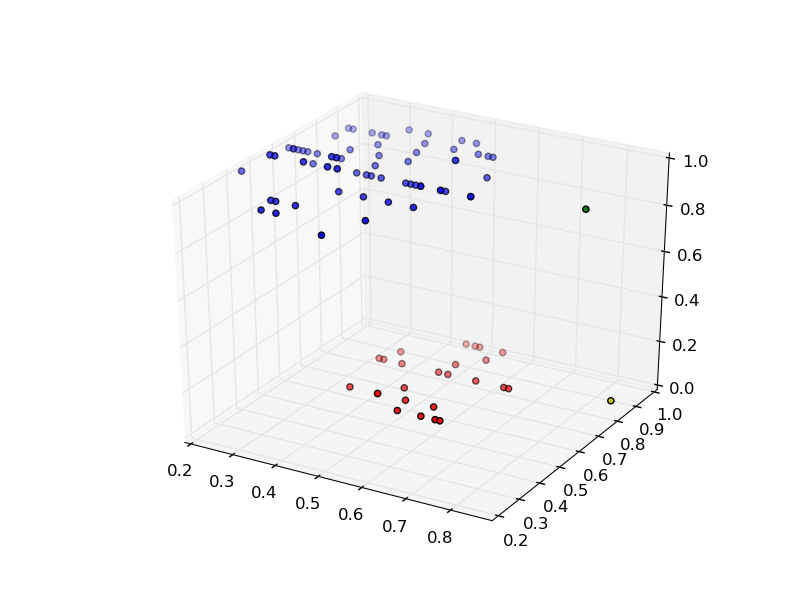
\includegraphics[height=2in]{scatter_metric0.png}

Scatterplot of Max metric clusters:

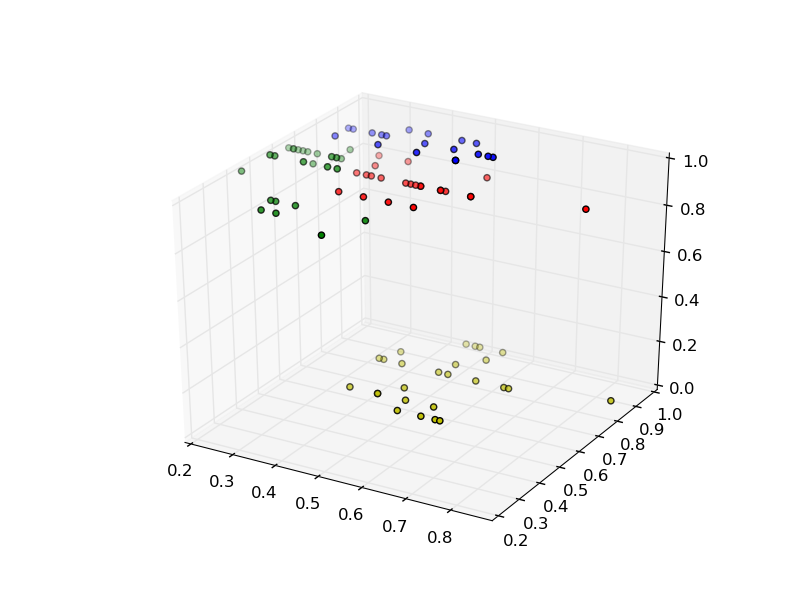
\includegraphics[height=2in]{scatter_metric1.png}

\item[(b)]
Number of instances in each cluster by metric:

 \begin{tabular}{ccc}
  Cluster Number&mean metric &centroid metric\\
 0&73&9\\
 1&25&89\\
 2&1&1\\
 3&1&1\\
 \end{tabular}

Scatterplot of mean metric clusters:

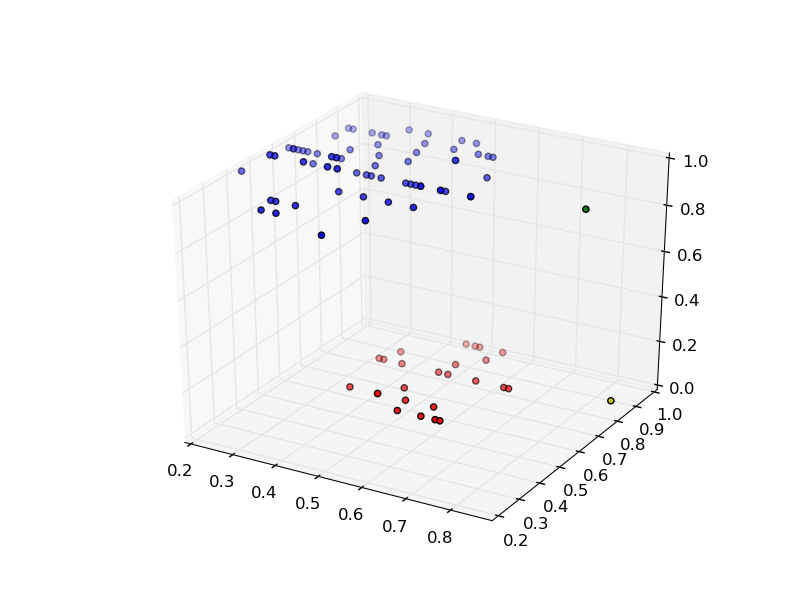
\includegraphics[height=2in]{scatter_metric2.png}

Scatterplot of centroid metric clusters:

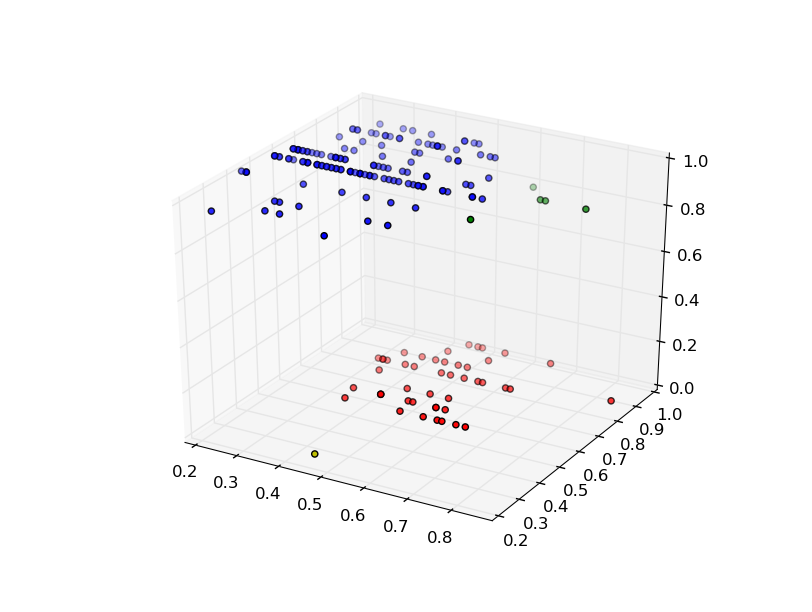
\includegraphics[height=2in]{scatter_metric3.png}

\end{enumerate}

\item[c.]
\begin{enumerate}
\item[(a)]
It takes autoclass 18 iterations to converge.

\item[(b)]

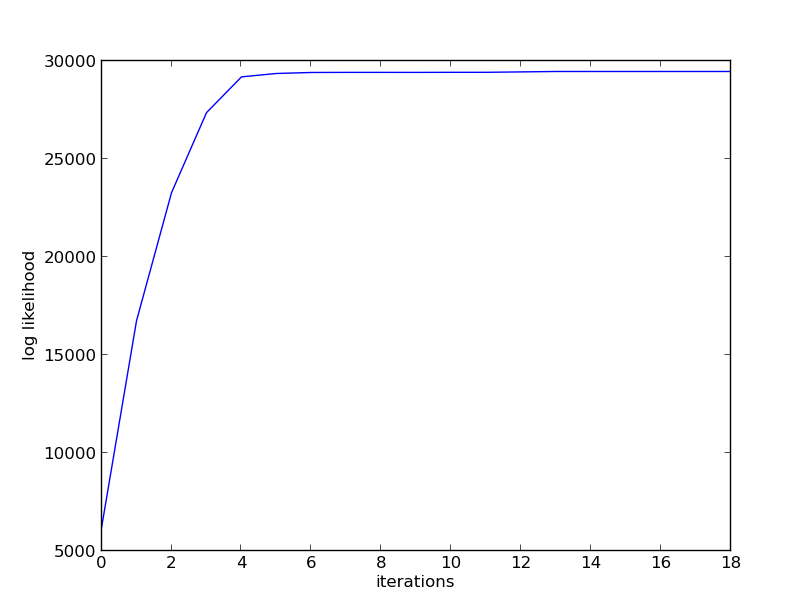
\includegraphics[height=2in]{log-likelihood.png}

\item[(c)]

0: 239
1: 394
2: 363
3: 4

\end{enumerate}

\end{enumerate}

\end{document}



